\chapter{Avances de implementación y prototipo inicial}
El presente capítulo describe los avances realizados durante la primera fase de desarrollo del sistema Graphito. Estos avances tienen como propósito demostrar la viabilidad técnica de la arquitectura propuesta y disminuir los módulos a desarrollar durante TT-2 para enfocar nuestros esfuerzos en los modulos de aprendizaje profundo, dividiendo los esfuerzos de implementación en dos áreas críticas: la construcción del prototipo de la capa de presentación y el establecimiento del pipeline de ingeniería de datos para los modelos de inteligencia artificial.

\section{Desarrollo de la Capa de Presentación (Front-end)}

La capa de presentación de Graphito se implementó como una Aplicación de Página Única (SPA) orientada a ofrecer una experiencia interactiva y de alto rendimiento. Su arquitectura interna sigue una estructura modular dividida en páginas, componentes reutilizables de interfaz y utilidades de diseño.

El ecosistema tecnológico base seleccionado para este desarrollo se detalla en el Cuadro \ref{tab:tech-stack}:

\begin{table}[H]
    \centering
    \caption{Tecnologías empleadas en el desarrollo del \textit{front-end}.}
    \begin{tabular}{|l|l|}
        \hline
        \textbf{Tecnología} & \textbf{Rol en la Arquitectura} \\ \hline
        React \& TypeScript & Biblioteca de componentes UI con tipado estático estricto. \\ \hline
        Vite & Entorno de desarrollo rápido y empaquetador de módulos. \\ \hline
        Tailwind CSS & \textit{Framework} de estilos utilitarios para maquetación ágil. \\ \hline
        GSAP & Motor de animaciones para transiciones fluidas en modales. \\ \hline
    \end{tabular}
    \label{tab:tech-stack}
\end{table}

El diseño de la plataforma obedece a una estética oscura con elementos translúcidos (\textit{glassmorphism}) para evocar un entorno de precisión técnica. Además, se implementó una jerarquía semántica de colores para comunicar de forma visual los niveles de riesgo de similitud detectados: rojo para niveles críticos ($>70\%$), ámbar para niveles medios ($30\%-70\%$) y azul para rangos seguros ($<30\%$).

\subsection{Componentes Generados}

Para consolidar la interfaz, se desarrollaron diversos componentes atómicos y estructurales que garantizan la consistencia visual y la reusabilidad del código:

\begin{itemize}
    \item \textbf{Componentes Estructurales:} Barra de navegación (\textit{Header}), contenedores translúcidos modulares (\textit{AuthCard}) y un fondo interactivo animado de alto impacto visual (\textit{MouseGlowBackground}).
    \item \textbf{Componentes Funcionales:} Tarjetas de referencias (\textit{ReferenceCard}) con acordeones desplegables, barras de búsqueda (\textit{SearchBar}) con filtrado en tiempo real, botones de llamado a la acción con degradados dinámicos (\textit{GradientButton}) y controles de paginación (\textit{PaginationControls}).
\end{itemize}

\section{Interfaces del Prototipo Inicial}

A continuación, se presentan las pantallas principales que conforman el flujo de auditoría académica del prototipo, ilustrando la integración de los componentes previamente descritos.

\begin{figure}[H]
    \centering
    % Descomenta la siguiente línea y reemplaza con tu imagen
    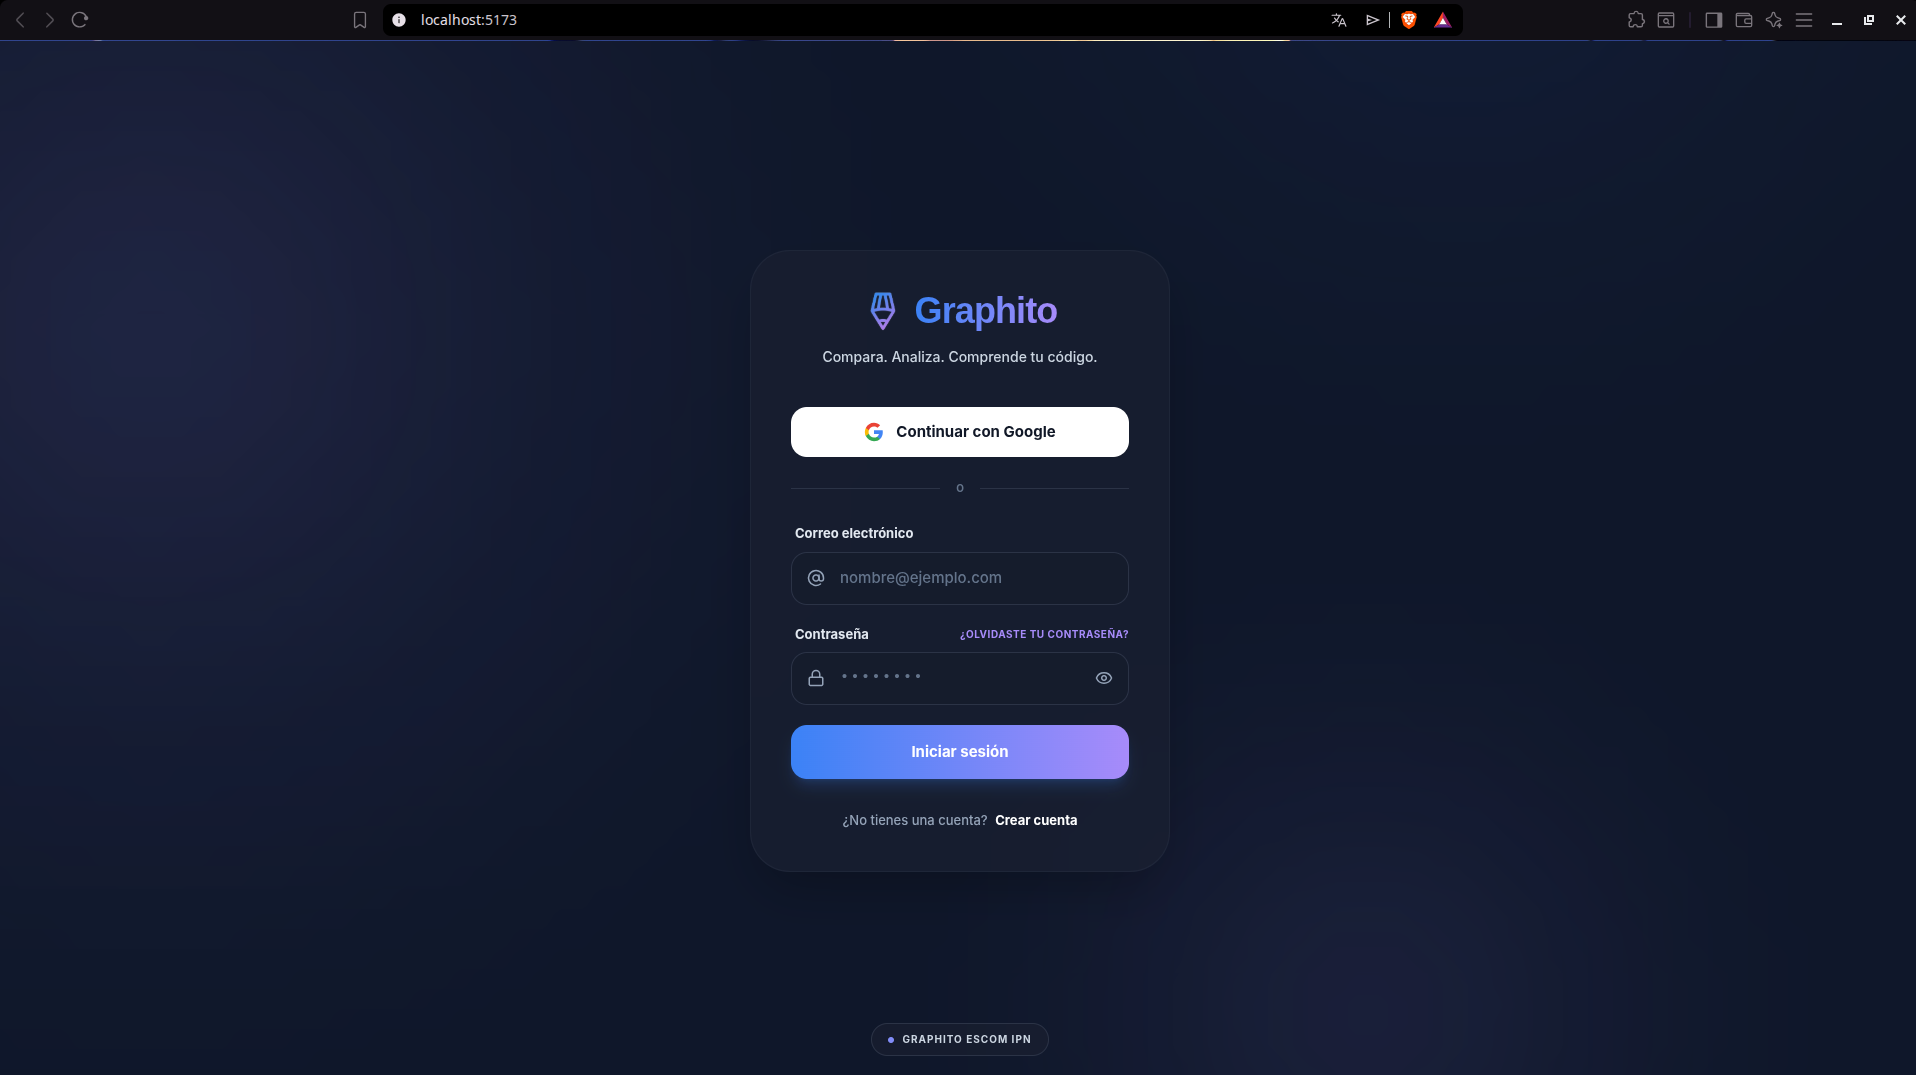
\includegraphics[width=0.85\textwidth]{img/login.png}
    \caption{Módulo de acceso seguro y registro para docentes. Implementa autenticación mediante credenciales estándar y servicios de terceros (OAuth).}
    \label{fig:ui-login}
\end{figure}

\begin{figure}[H]
    \centering
    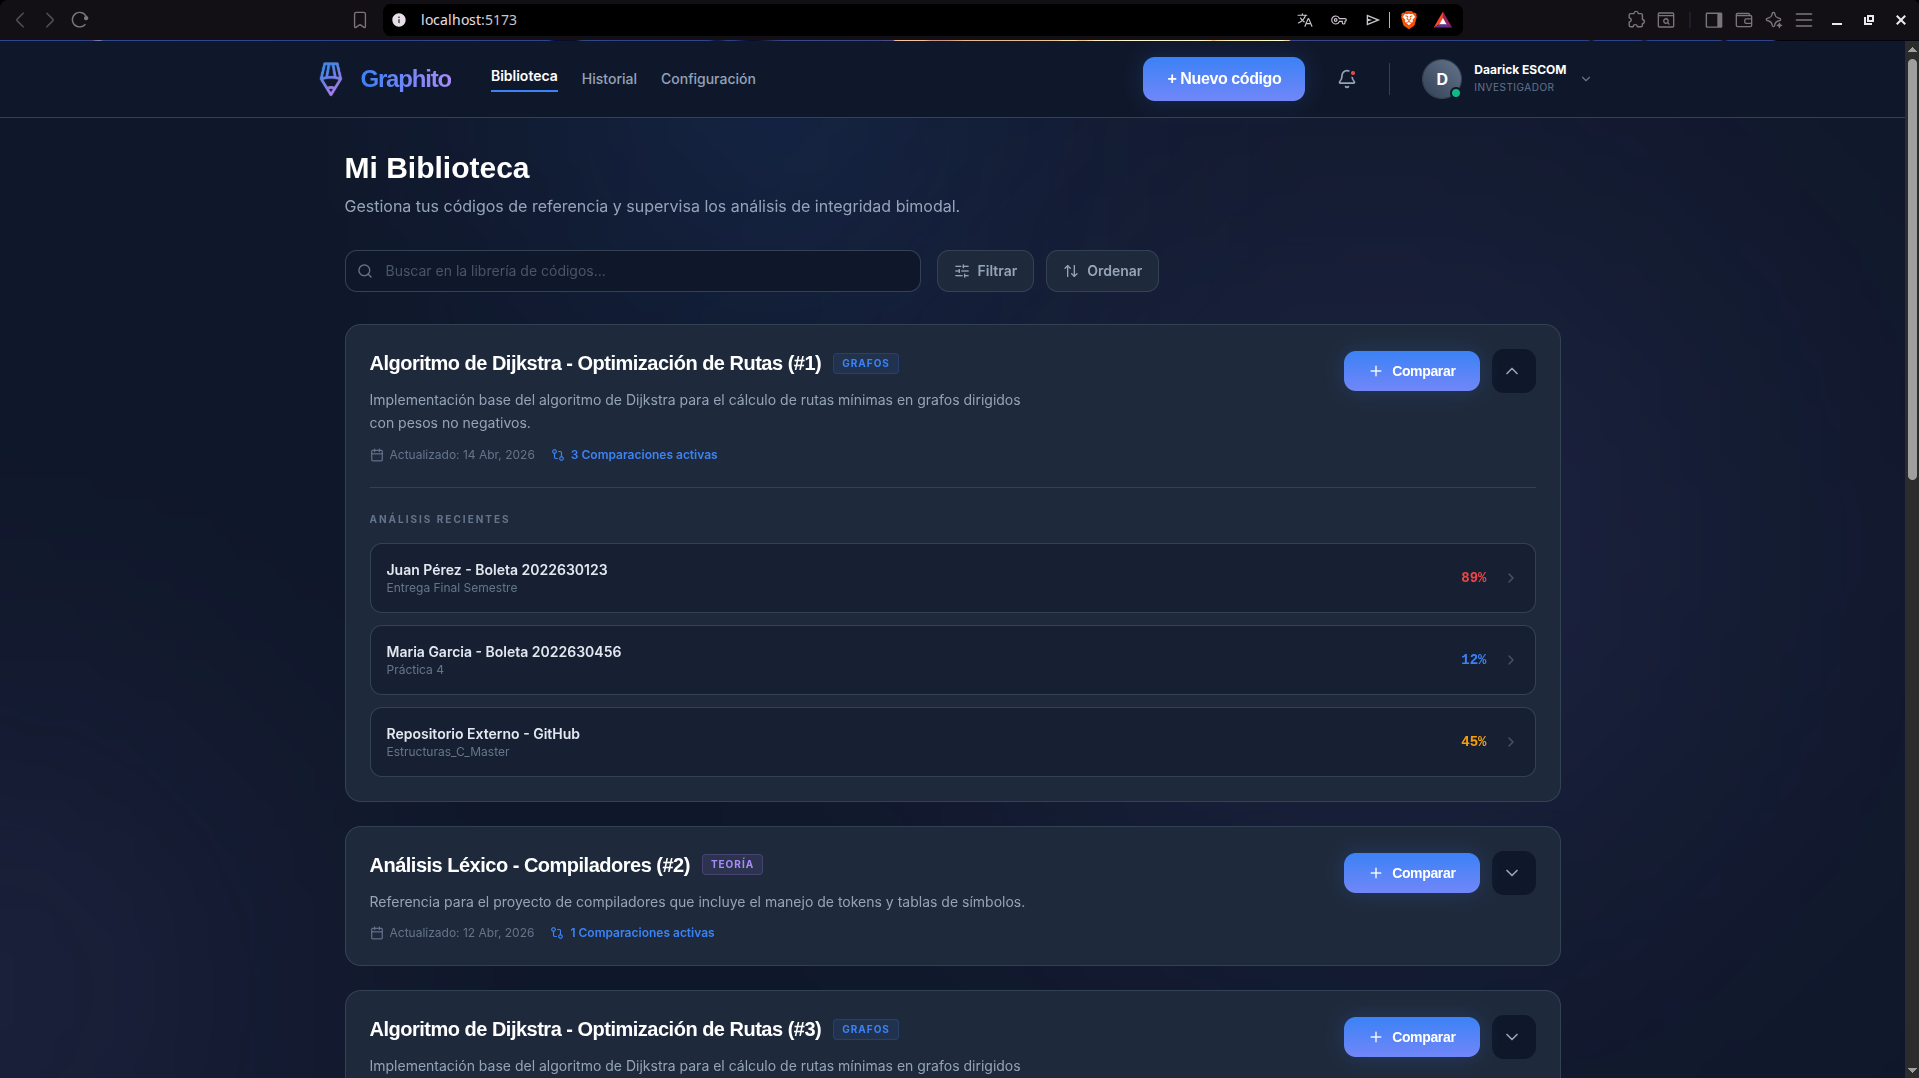
\includegraphics[width=0.85\textwidth]{img/biblioteca.png}
    \caption{Dashboard del docente. Despliega el repositorio de ejercicios gestionados, controles de búsqueda y el resumen histórico de las comparaciones realizadas.}
    \label{fig:ui-biblioteca}
\end{figure}

\begin{figure}[H]
    \centering
    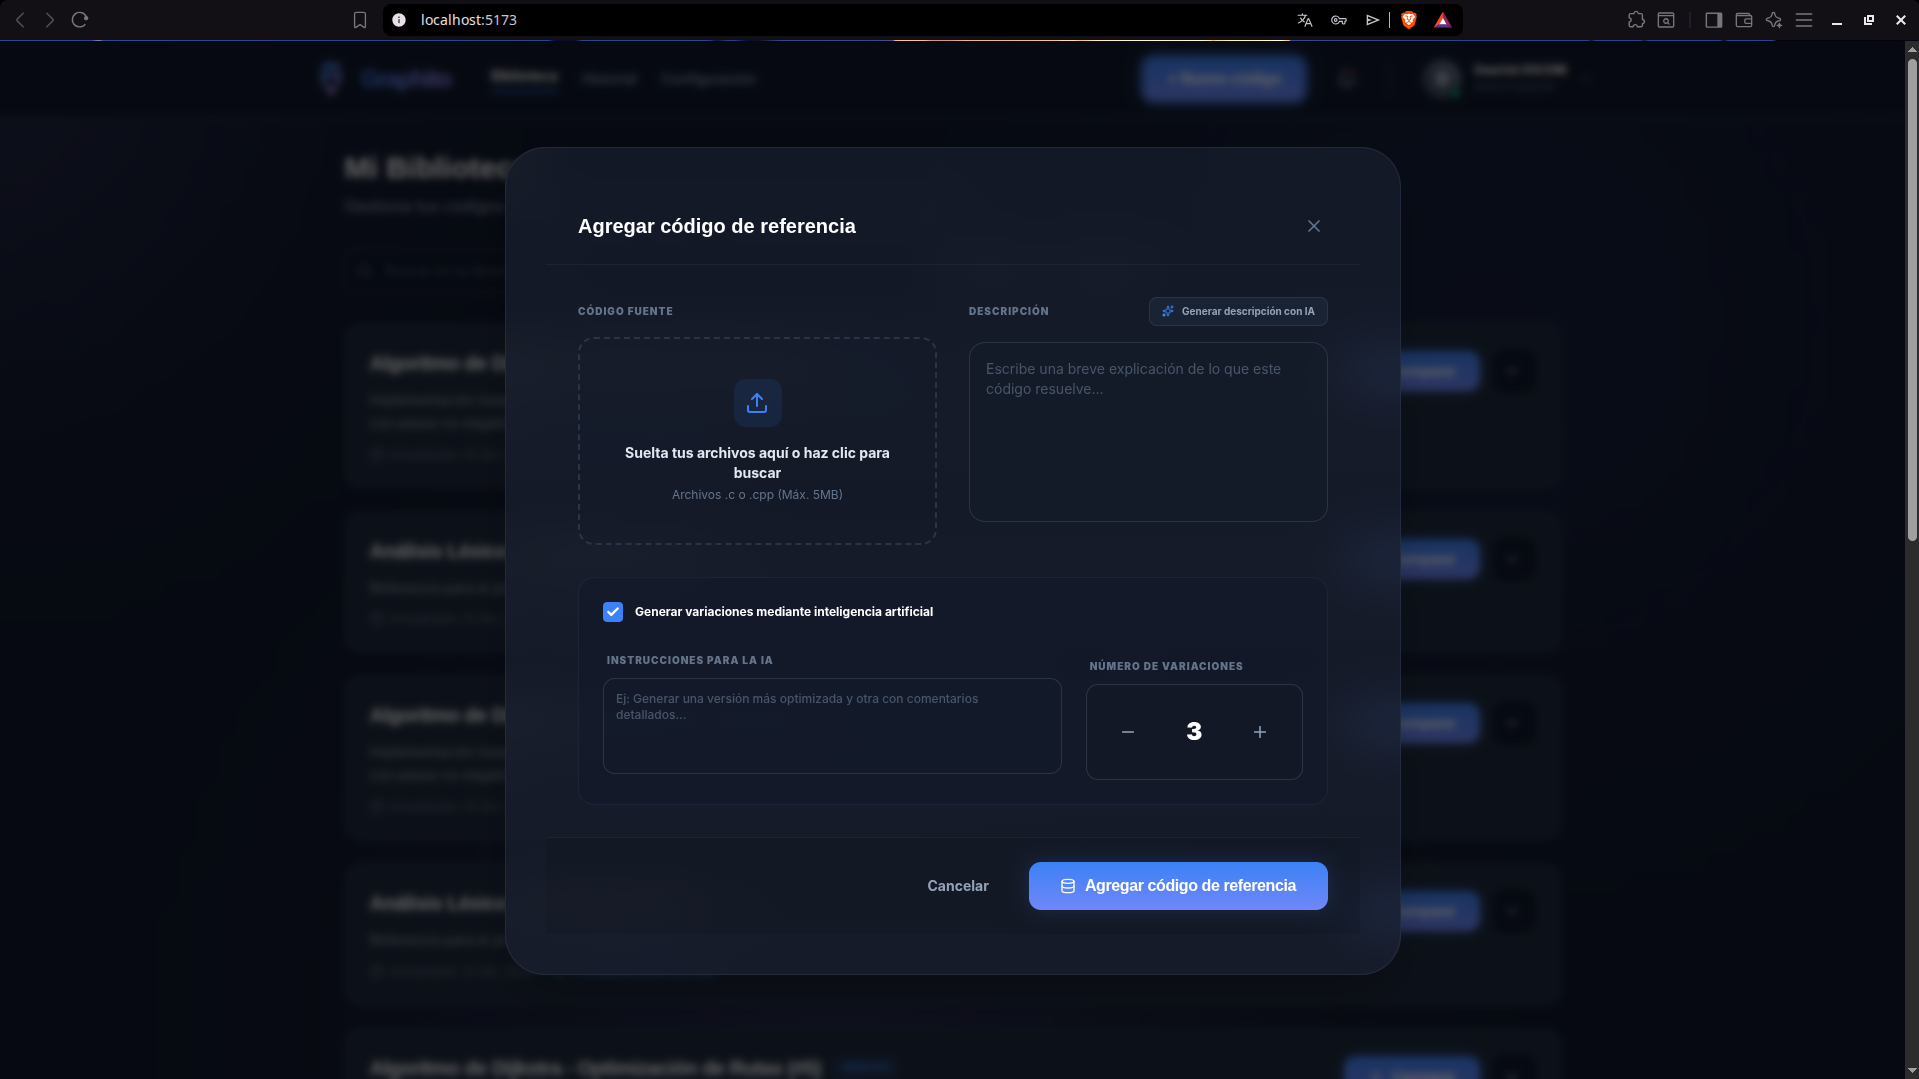
\includegraphics[width=0.85\textwidth]{img/referencia.png}
    \caption{Interfaz para la carga del código de referencia. Incluye las herramientas de parametrización para la generación de variantes y descripciones técnicas asistidas por Inteligencia Artificial.}
    \label{fig:ui-modal-referencia}
\end{figure}

\begin{figure}[H]
    \centering
    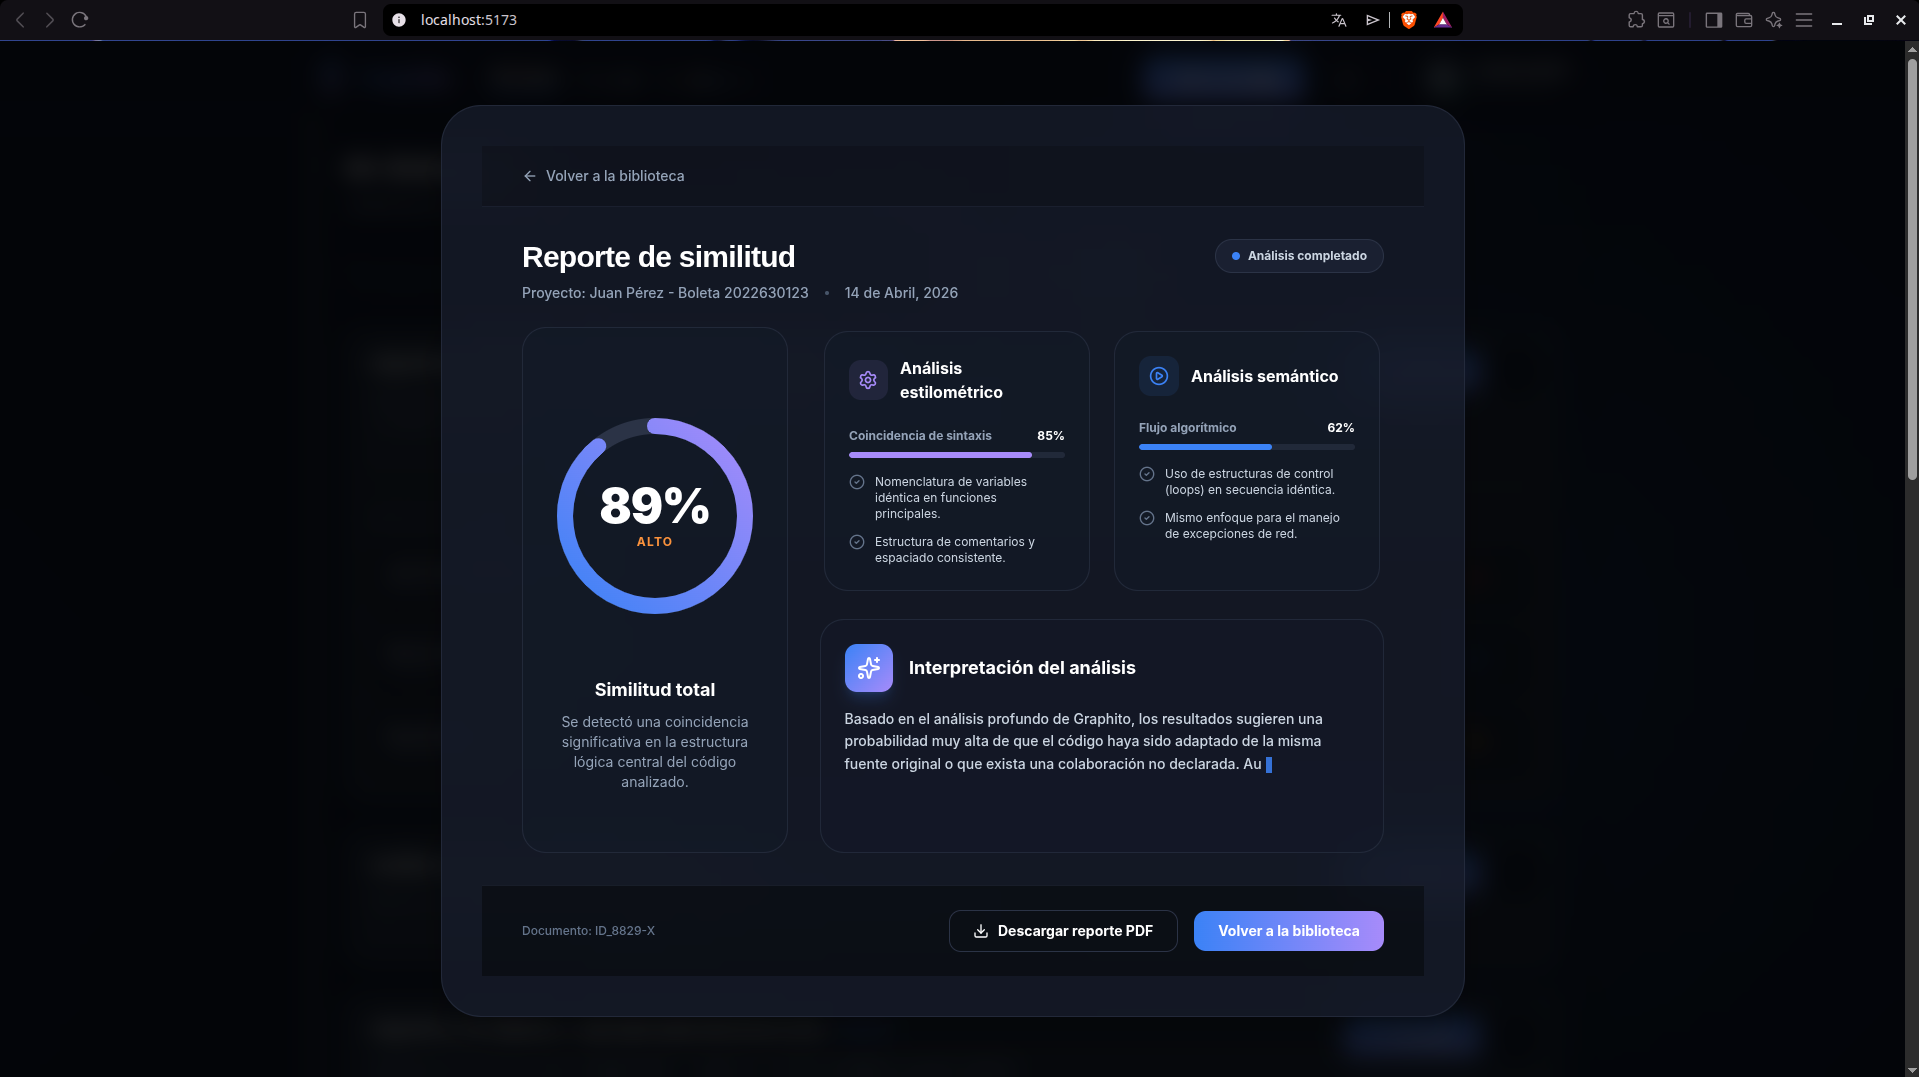
\includegraphics[width=0.85\textwidth]{img/reporte.png}
    \caption{Panel interactivo del reporte de integridad. Renderiza los gráficos circulares de la similitud semántica y estilométrica, junto a la interpretación del reporte.}
    \label{fig:ui-reporte}
\end{figure}

\section{Ingeniería de Datos y Preparación del conjunto de datos}

De forma paralela al desarrollo del \textit{software}, se ejecutaron las fases iniciales de la metodología correspondiente a la Adquisición, Exploración y Preparación de Datos. La conformación de un corpus robusto y balanceado es un requisito indispensable para el posterior entrenamiento del clasificador estilométrico (CharCNN).

\subsection{Exploración del Dataset IEEE Plagiarism}

Para la recolección de la clase correspondiente al código humano, se seleccionó el \textit{dataset IEEE Plagiarism}, un repositorio académico que contiene entregas reales de estudiantes universitarios programadas en C y C++. 

Como resultado de esta fase de análisis exploratorio, se documentó la estructura interna de los directorios, los cuales están agrupados por curso, asignación y problema. Las dimensiones cuantitativas y características técnicas identificadas en el conjunto de datos original se resumen en el Cuadro \ref{tab:dimensiones-dataset}:

\begin{table}[H]
    \centering
    \caption{Dimensiones generales y características operativas del dataset IEEE Plagiarism.}
    \begin{tabular}{|l|l|}
        \hline
        \textbf{Dimensión} & \textbf{Valor} \\ \hline
        Cursos analizados & 4 (A2016, A2017, B2016, B2017) \\ \hline
        Lenguaje de programación & C / C++ \\ \hline
        Volumen de estudiantes & $\sim$100-150 por curso \\ \hline
        Asignaciones evaluadas & 16-22 por curso \\ \hline
        Formato de trazas del IDE & JSON (registro de eventos) \\ \hline
        Anonimización de datos & Nombres reemplazados por \texttt{student\{id\}} \\ \hline
    \end{tabular}
    \label{tab:dimensiones-dataset}
\end{table}

Si bien el conjunto de datos proporciona un volumen sustancial de código humano etiquetado para el análisis de similitud, la exploración reveló una carencia metodológica crítica: el \textit{dataset} no incluía los enunciados técnicos originales ni las instrucciones que detallaban los requerimientos algorítmicos de cada problema. Esta ausencia representaba un obstáculo para la posterior generación de código sintético, ya que los modelos generativos requieren un \textit{prompt} preciso para simular soluciones funcionalmente equivalentes.

\subsection{Ingeniería Inversa y Recuperación de Enunciados}

Para solucionar esta carencia, se diseñó y ejecutó un \textit{script} automatizado en Python (\texttt{extraer\_enunciados.py}) capaz de realizar ingeniería inversa sobre el código de los estudiantes. El proceso integra un Modelo de Lenguaje de Gran Escala (LLM) que analiza una muestra representativa de entregas humanas por cada clúster de problemas, deduciendo y redactando el enunciado original. 

Este proceso incluyó mecanismos de resiliencia, como la generación de puntos de control (\textit{checkpoints}), y culminó exitosamente con la consolidación de un archivo estructurado (\texttt{enunciados.csv}). Este archivo contiene la metainformación recuperada, sirviendo como catálogo base para la siguiente etapa del proyecto.

Como evidencia empírica de la efectividad de este proceso, en el Cuadro \ref{tab:ejemplos-enunciados} se presenta una muestra de los requerimientos deducidos automáticamente por el modelo.

\begin{table}[H]
    \centering
    \caption{Muestra de enunciados extraídos mediante ingeniería inversa sobre el código de los estudiantes.}
    \renewcommand{\arraystretch}{1.3} % Añade espacio vertical para mejorar la legibilidad
    \small % Reduce ligeramente el tamaño de la fuente para ajustar el texto
    \begin{tabular}{|c|c|c|c|p{8.5cm}|}
        \hline
        \textbf{Curso} & \textbf{Asig.} & \textbf{Prob.} & \textbf{Leng.} & \textbf{Enunciado Inferido} \\ \hline
        A2016 & Z1 & Z1 & C & Calcular la suma de los puntos obtenidos por tres estudiantes (Tarik, Bojan y Mirza) en una asignatura, basándose en los resultados de cinco categorías: primer examen parcial (máximo 20 pts), segundo examen parcial (máximo 20 pts), asistencia (máximo 10 pts), tareas (máximo 10 pts) y examen final (máximo 40 pts). El programa debe validar que las entradas estén dentro de los rangos permitidos y finalizar con un mensaje de error si algún valor es inválido. \\ \hline
        A2016 & Z1 & Z2 & C & Dados los coeficientes de dos rectas en la forma $y = ax + b$ ($y_1 = a_1x + b_1$ y $y_2 = a_2x + b_2$), determinar su posición relativa (paralelas, coincidentes o secantes) y, en caso de ser secantes, calcular las coordenadas del punto de intersección. \\ \hline
        A2016 & Z1 & Z3 & C & Escriba un programa que permita ingresar una serie de caracteres que representan los colores de vehículos (c: negro, b: blanco, s: gris, v: rojo, p: azul). El ingreso finaliza al introducir el carácter 'k'. El programa debe contar el total de vehículos ingresados, calcular el porcentaje de cada color y determinar cuál es el color más popular (en caso de empate, gana el que apareció primero). \\ \hline
        A2016 & Z1 & Z4 & C & Escribir un programa que solicite al usuario un número entero $n$ (donde $0 < n \leq 50$) e imprima en pantalla una letra 'W' (o un patrón de estrella en forma de W) formada por asteriscos, con una altura de $n$ filas. \\ \hline
    \end{tabular}
    \label{tab:ejemplos-enunciados}
\end{table}

Como se puede observar en la muestra, el modelo de lenguaje no solo identificó el propósito general del código, sino que logró extraer de manera precisa reglas de negocio específicas (como los límites de puntuación del problema Z1), condiciones lógicas (criterios de desempate en Z3) y fórmulas matemáticas (ecuaciones de la recta en Z2). Esta precisión semántica es un hito fundamental para la ingeniería de datos del proyecto, ya que garantiza que las referencias sintéticas que se generen posteriormente resuelvan de manera estricta el mismo problema algorítmico que las entregas humanas, eliminando el sesgo por ambigüedad.
\subsection{Diseño del Pipeline para la Clase Sintética}

Una vez superada la limitación de los enunciados, se procedió a diseñar y programar la arquitectura lógica para la generación de la clase sintética, sentando las bases tecnológicas para la siguiente fase del Trabajo Terminal.

Se desarrolló un \textit{pipeline} modular en Python (\texttt{generar\_referencias.py}) que interactúa de manera agnóstica con múltiples proveedores de Inteligencia Artificial mediante una capa de abstracción. La herramienta está preparada para consumir el archivo \texttt{enunciados.csv} y solicitar la resolución algorítmica a modelos estado del arte (SOTA) a través de APIs (tales como OpenAI y Anthropic), así como a modelos de código abierto ejecutados localmente (vía Ollama). 

Si bien la ejecución masiva para la generación de referencias sintéticas forma parte de las actividades planificadas para las etapas posteriores de validación y entrenamiento, el ecosistema de \textit{scripts} y la ingeniería de datos subyacente se encuentran completamente operativos e integrados para comenzar con la recolección de código sintético a la brevedad y contar con tiempo suficiente para realizar pruebas y entrenar el modelo de CharCNN.

\section{Conclusión del capítulo}

Los avances descritos en este capítulo representan la base operativa y funcional sobre la cual se erige el sistema Graphito. La implementación anticipada del prototipo de interfaz y la automatización del flujo de datos mediante \textit{scripts} especializados responden a un enfoque estratégico de optimización de tiempos de desarrollo. 

Al haber consolidado la capa de presentación y el ecosistema de ingeniería de datos en esta etapa inicial, se logra reducir significativamente la carga operativa de las fases posteriores. Esto garantiza que, durante el desarrollo de la segunda parte del Trabajo Terminal, los esfuerzos técnicos y analíticos puedan concentrarse prioritariamente en los módulos fundamentales y de mayor complejidad científica: el entrenamiento, ajuste fino y validación de los modelos de inteligencia artificial (GraphCodeBERT y CharCNN). De este modo, la arquitectura del sistema queda preparada para evolucionar de un prototipo funcional a una herramienta de auditoría académica robusta y de alto rendimiento.